% !TEX program = xelatex
\documentclass[a4paper,10pt]{article}
\usepackage[UTF8,fontset=none]{ctex}
\usepackage{xeCJK}
\setCJKmainfont{Songti SC}
\setCJKsansfont{STHeiti}
\setCJKmonofont{Songti SC}
\usepackage[margin=2.2cm]{geometry}
\usepackage{tikz}
\usetikzlibrary{shapes.geometric, arrows.meta, positioning, calc, fit}
\usepackage{amsmath, amssymb}
\usepackage{longtable}
\usepackage{array}
\usepackage{booktabs}
\usepackage{multirow}
\usepackage{enumitem}
\usepackage{fancyhdr}
\usepackage{titlesec}
\usepackage{hyperref}
\usepackage{xcolor}
\usepackage{tabularx}

\hypersetup{
  colorlinks=true,
  linkcolor=blue!60!black,
  urlcolor=blue!60!black,
  bookmarksnumbered=true
}

% 页眉页脚
\pagestyle{fancy}
\fancyhf{}
\fancyhead[L]{\small 路点跟踪MPC控制器~---~设计文档}
\fancyhead[R]{\small 内部公开}
\fancyfoot[C]{\thepage}
\renewcommand{\headrulewidth}{0.4pt}

% 层级编号
\setcounter{secnumdepth}{3}
\setcounter{tocdepth}{3}

% 表格列宽辅助
\newcolumntype{L}[1]{>{\raggedright\arraybackslash}p{#1}}
\newcolumntype{C}[1]{>{\centering\arraybackslash}p{#1}}

% ============================================================
\begin{document}

% ==================== 封面表格 ====================
\thispagestyle{empty}

\begin{center}
{\CJKfamily{zhsong}\bfseries\Large 函数设计文档}
\end{center}

\vspace{8pt}

\begin{center}
\renewcommand{\arraystretch}{1.5}
\begin{tabular}{|L{3.2cm}|L{4.5cm}|L{3.2cm}|L{4.5cm}|}
\hline
\textbf{函数英文名} & waypointFollow &
\textbf{函数中文名} & 路点跟踪MPC控制器 \\
\hline
\textbf{函数类型} & 组件 (Component) &
\textbf{版本} & 2.0 \\
\hline
\textbf{作者} & 许庆 &
\textbf{日期} & 2026-06-26 \\
\hline
\textbf{联系方式} & \multicolumn{3}{l|}{18612426814~/~qingxu@tsinghua.edu.cn} \\
\hline
\textbf{密级} & 内部公开 &
\textbf{AI辅助} & Cursor Agent (Claude Opus 4.6) \\
\hline
\end{tabular}
\end{center}

\vspace{12pt}

\begin{center}
\renewcommand{\arraystretch}{1.4}
\begin{tabular}{|C{1.2cm}|C{2cm}|L{5cm}|C{2cm}|C{2cm}|}
\hline
\multicolumn{5}{|c|}{\textbf{更改记录}} \\
\hline
\textbf{版本} & \textbf{日期} & \textbf{更改说明} & \textbf{作者} & \textbf{审核} \\
\hline
1.0 & 2026-06-20 & 初始版本：单步梯度优化 & 许庆 & --- \\
\hline
2.0 & 2026-06-26 & 重构为多步MPC + 暖启动 + 自适应步长 & 许庆 & --- \\
\hline
\end{tabular}
\end{center}

\newpage

% ==================== 目录 ====================
\tableofcontents
\newpage

% ============================================================
%  1. 函数需求
% ============================================================
\section{函数需求}

\subsection{功能概述}

\texttt{waypointFollow} 实现基于模型预测控制（MPC）的路点跟踪控制器。
给定自车车速、当前方向盘转角以及未来 6 个参考路点（对应 0.5\,s -- 3.0\,s），
控制器输出期望的方向盘转角和纵向加速度，使车辆沿参考路点行驶。

\subsection{功能需求}

\begin{enumerate}[label=FR-\arabic*]
  \item 对 6 个参考路点附加原点后进行 X 归一化三次多项式最小二乘拟合，生成平滑参考轨迹。
  \item 基于运动学自行车模型进行多步状态预测。
  \item 构造包含轨迹跟踪误差、控制幅值、控制变化率的二次代价函数。
  \item 采用中心差分数值梯度 + 自适应步长梯度下降迭代优化控制序列。
  \item 支持暖启动：利用上一周期优化结果初始化当前周期控制序列。
  \item 低速保护：车速低于 0.5\,m/s 时保持当前转向并输出零加速度。
  \item 输出限幅保护：转向角和加速度不超过物理约束。
\end{enumerate}

\subsection{非功能需求}

\begin{enumerate}[label=NFR-\arabic*]
  \item 代码不使用动态内存分配，所有数组大小编译期确定，适用于嵌入式场景。
  \item 不依赖第三方数值库，全部算法自包含。
  \item 单周期计算时间应满足 100\,ms 实时约束（典型 10\,Hz 控制频率）。
\end{enumerate}

% ============================================================
%  2. 算法设计
% ============================================================
\section{算法设计}

\subsection{整体流程}

控制器每个周期执行以下步骤：
\begin{enumerate}
  \item 方向盘转角除以传动比，换算为前轮转角 $\delta_{\text{front}} = \theta_{\text{sw}} / r_{\text{steer}}$。
  \item 低速检测：若 $v < 0.5$\,m/s，直接输出零控制。
  \item 初始化暖启动序列（首次调用时）。
  \item 调用 \texttt{fitWaypointTrajectory} 拟合参考轨迹。
  \item 构造暖启动序列（将上一周期控制序列左移一步）。
  \item 调用 \texttt{mpcOptimize} 求解最优控制序列。
  \item 提取首步控制量，换算回方向盘转角并限幅输出。
  \item 更新暖启动状态。
\end{enumerate}

\subsection{路点轨迹拟合}

将原点 $(0,0)$ 和 6 个路点共 7 个数据点 $(x_i, y_i)$ 进行拟合。
首先对 X 坐标进行归一化：
\begin{equation}
  \bar{x}_i = \frac{x_i - x_{\min}}{x_{\max} - x_{\min}}, \quad i = 0, 1, \ldots, 6
\end{equation}

在归一化坐标系下进行三次多项式最小二乘拟合：
\begin{equation}
  y(\bar{x}) = c_0 + c_1 \bar{x} + c_2 \bar{x}^2 + c_3 \bar{x}^3
\end{equation}

构造 Vandermonde 矩阵 $\mathbf{A}$，各行为 $[1, \bar{x}_i, \bar{x}_i^2, \bar{x}_i^3]$，
求解法方程：
\begin{equation}
  (\mathbf{A}^{\!\top}\!\mathbf{A})\,\mathbf{c} = \mathbf{A}^{\!\top}\!\mathbf{y}
\end{equation}

法方程通过高斯消元法（部分主元选取）求解。

参考车速由路点间累计弧长除以总时间跨度（3.0\,s）估算：
\begin{equation}
  v_{\text{ref}} = \frac{\sum_{i=0}^{5} \|\mathbf{p}_{i+1} - \mathbf{p}_i\|}{3.0}
\end{equation}
其中 $\mathbf{p}_0 = (0,0)$。

\subsection{运动学自行车模型}

采用前轮驱动运动学自行车模型，状态向量 $\mathbf{s} = [x, y, \psi, v]^{\!\top}$，
控制输入 $\mathbf{u} = [\delta, a]^{\!\top}$，连续时间方程为：
\begin{equation}
  \begin{cases}
    \dot{x} = v \cos\psi \\
    \dot{y} = v \sin\psi \\
    \dot{\psi} = \dfrac{v \tan\delta}{L} \\
    \dot{v} = a
  \end{cases}
\end{equation}
其中 $L$ 为轴距。采用欧拉前向离散化，步长 $\Delta t$：
\begin{equation}
  \begin{cases}
    x_{k+1} = x_k + v_k \cos\psi_k \cdot \Delta t \\
    y_{k+1} = y_k + v_k \sin\psi_k \cdot \Delta t \\
    \psi_{k+1} = \psi_k + \dfrac{v_k \tan\delta_k}{L} \cdot \Delta t \\
    v_{k+1} = v_k + a_k \cdot \Delta t
  \end{cases}
\end{equation}

\subsection{MPC代价函数}

设预测时域 $N_p$，控制时域 $N_c$（$N_c \leq N_p$）。
超出控制时域后控制量保持 $\mathbf{u}_{N_c-1}$ 不变。代价函数为：
\begin{equation}
  J = \underbrace{\sum_{k=1}^{N_p} \Big( w_{\text{lat}} e_{y,k}^2 + w_{\text{head}} e_{\psi,k}^2 + w_{v} e_{v,k}^2 \Big)}_{\text{轨迹跟踪代价}}
    + \underbrace{\sum_{k=0}^{N_c-1} \Big( w_\delta \delta_k^2 + w_a a_k^2 \Big)}_{\text{控制幅值代价}}
    + \underbrace{\sum_{k=0}^{N_c-1} \Big( w_{\Delta\delta} \Delta\delta_k^2 + w_{\Delta a} \Delta a_k^2 \Big)}_{\text{控制变化率代价}}
\end{equation}
其中：
\begin{itemize}
  \item $e_{y,k} = y_k - y_{\text{ref}}(\bar{x}_k)$：横向偏差
  \item $e_{\psi,k} = \text{normalize}(\psi_k - \psi_{\text{ref},k})$：航向偏差，
        $\psi_{\text{ref},k} = \arctan\!\Big(\dfrac{dy/d\bar{x}}{x_{\text{scale}}}\Big)$
  \item $e_{v,k} = v_k - v_{\text{ref}}$：速度偏差
  \item $\Delta\delta_k = \delta_k - \delta_{k-1}$，$\Delta a_k = a_k - a_{k-1}$（$k{=}0$ 时取上周期值）
\end{itemize}

\subsection{梯度下降优化}

\subsubsection{数值梯度计算}

对控制序列中的每个分量 $u_i$ 采用中心差分计算梯度：
\begin{equation}
  \frac{\partial J}{\partial u_i} \approx \frac{J(u_i + \varepsilon) - J(u_i - \varepsilon)}{2\varepsilon},
  \quad \varepsilon = 10^{-3}
\end{equation}

\subsubsection{梯度归一化与参数更新}

计算梯度范数的平方 $\|\nabla J\|^2 = \sum_i g_i^2$，
对梯度进行归一化缩放以防止更新过大：
\begin{equation}
  s = \frac{1}{1 + \|\nabla J\|^2}
\end{equation}
参数更新规则：
\begin{equation}
  u_i^{(t+1)} = u_i^{(t)} - \alpha \cdot g_i \cdot s
\end{equation}
其中 $\alpha$ 为自适应学习率。

\subsubsection{自适应步长与约束}

\begin{itemize}
  \item 若候选控制序列的代价 $J_{\text{new}} < J_{\text{old}}$，接受更新。
  \item 否则拒绝更新，将学习率衰减为原来的 $0.5$ 倍。
  \item 每步更新后施加幅值约束 $|\delta| \leq \delta_{\max}$，$a_{\min} \leq a \leq a_{\max}$。
  \item 施加转向角变化率约束 $|\delta_k - \delta_{k-1}| \leq \Delta\delta_{\max}$。
\end{itemize}

% ============================================================
%  3. 程序流程图
% ============================================================
\section{程序流程图}

\begin{center}
\begin{tikzpicture}[
  node distance=1.0cm and 1.5cm,
  startstop/.style={rectangle, rounded corners, minimum width=3.5cm, minimum height=0.7cm,
    text centered, draw=black, fill=blue!8, font=\small},
  process/.style={rectangle, minimum width=4.5cm, minimum height=0.7cm,
    text centered, draw=black, fill=orange!8, font=\small},
  decision/.style={diamond, aspect=2.2, minimum width=2cm,
    text centered, draw=black, fill=green!8, font=\small},
  io/.style={trapezium, trapezium left angle=70, trapezium right angle=110,
    minimum width=3.5cm, minimum height=0.7cm,
    text centered, draw=black, fill=yellow!8, font=\small},
  arrow/.style={-{Stealth[length=2.5mm]}, thick}
]

\node (start) [startstop] {开始};
\node (input) [io, below=of start] {读入 egoSpeed, steeringWheelAngle, waypoints};
\node (convert) [process, below=of input] {方向盘转角 $\to$ 前轮转角};
\node (lowspd) [decision, below=of convert] {$v < 0.5$\,m/s?};
\node (lowout) [process, right=2.5cm of lowspd] {输出零控制};
\node (initchk) [decision, below=of lowspd] {已初始化?};
\node (initwarm) [process, right=2.5cm of initchk] {初始化暖启动序列};
\node (fit) [process, below=of initchk] {fitWaypointTrajectory};
\node (fitchk) [decision, below=of fit] {拟合有效?};
\node (fitfail) [process, right=2.5cm of fitchk] {输出零控制};
\node (warm) [process, below=of fitchk] {构造暖启动序列(左移)};
\node (mpc) [process, below=of warm] {mpcOptimize};
\node (extract) [process, below=of mpc] {提取首步控制量};
\node (clamp) [process, below=of extract] {限幅保护};
\node (update) [process, below=of clamp] {更新暖启动状态};
\node (output) [io, below=of update] {输出 steeringWheelAngle, acceleration};
\node (stop) [startstop, below=of output] {结束};

\draw [arrow] (start) -- (input);
\draw [arrow] (input) -- (convert);
\draw [arrow] (convert) -- (lowspd);
\draw [arrow] (lowspd) -- node[above]{\small 是} (lowout);
\draw [arrow] (lowout) |- (output);
\draw [arrow] (lowspd) -- node[right]{\small 否} (initchk);
\draw [arrow] (initchk) -- node[above]{\small 否} (initwarm);
\draw [arrow] (initwarm) |- ([yshift=-0.2cm]initchk.south) -- (fit);
\draw [arrow] (initchk) -- node[right]{\small 是} (fit);
\draw [arrow] (fit) -- (fitchk);
\draw [arrow] (fitchk) -- node[above]{\small 否} (fitfail);
\draw [arrow] (fitfail) |- (output);
\draw [arrow] (fitchk) -- node[right]{\small 是} (warm);
\draw [arrow] (warm) -- (mpc);
\draw [arrow] (mpc) -- (extract);
\draw [arrow] (extract) -- (clamp);
\draw [arrow] (clamp) -- (update);
\draw [arrow] (update) -- (output);
\draw [arrow] (output) -- (stop);

\end{tikzpicture}
\end{center}

% ============================================================
%  4. 函数接口与输入输出模块图
% ============================================================
\section{函数接口与输入输出模块图}

\begin{center}
\begin{tikzpicture}[
  box/.style={rectangle, draw=black, thick, minimum width=3.5cm, minimum height=0.7cm,
    text centered, fill=blue!6, font=\small},
  core/.style={rectangle, draw=black, very thick, minimum width=5cm, minimum height=2.2cm,
    text centered, fill=orange!10, font=\normalsize\bfseries, rounded corners=3pt},
  iobox/.style={rectangle, draw=black, thick, minimum width=3.0cm, minimum height=0.6cm,
    text centered, fill=yellow!10, font=\small},
  arrow/.style={-{Stealth[length=2.5mm]}, thick}
]

% 核心模块
\node (core) [core] {waypointFollow};

% 输入 (左侧)
\node (in1) [iobox, left=3cm of core, yshift=1.2cm] {egoSpeed (m/s)};
\node (in2) [iobox, left=3cm of core, yshift=0.4cm] {steeringWheelAngle (rad)};
\node (in3) [iobox, left=3cm of core, yshift=-0.4cm] {waypoints[6] (x,y)};

% 参数 (上方)
\node (p1) [iobox, above=1.2cm of core, xshift=-1.8cm] {MpcParam};
\node (p2) [iobox, above=1.2cm of core, xshift=1.8cm] {steeringRatio};

% 状态 (下方)
\node (s1) [iobox, below=1.2cm of core, xshift=-2cm] {prevControlSequence[]};
\node (s2) [iobox, below=1.2cm of core, xshift=2cm] {lastAppliedControl};

% 输出 (右侧)
\node (out1) [iobox, right=3cm of core, yshift=0.4cm] {steeringWheelAngle (rad)};
\node (out2) [iobox, right=3cm of core, yshift=-0.4cm] {acceleration (m/s\textsuperscript{2})};

% 箭头
\draw [arrow] (in1) -- (core);
\draw [arrow] (in2) -- (core);
\draw [arrow] (in3) -- (core);
\draw [arrow] (p1) -- (core);
\draw [arrow] (p2) -- (core);
\draw [arrow, <->] (s1) -- (core);
\draw [arrow, <->] (s2) -- (core);
\draw [arrow] (core) -- (out1);
\draw [arrow] (core) -- (out2);

% 标签
\node [above=0.1cm of in1, font=\small\bfseries] {输入 (Input)};
\node [above=0.1cm of p1, xshift=1.8cm, font=\small\bfseries] {参数 (Param)};
\node [below=0.1cm of s1, xshift=2cm, font=\small\bfseries] {状态 (State)};
\node [above=0.1cm of out1, font=\small\bfseries] {输出 (Output)};

\end{tikzpicture}
\end{center}

% ============================================================
%  5. 函数诸元表
% ============================================================
\section{函数诸元表}

\renewcommand{\arraystretch}{1.3}
\begin{longtable}{|L{3.8cm}|L{11.5cm}|}
\hline
\textbf{属性} & \textbf{说明} \\
\hline
\endfirsthead
\hline
\textbf{属性} & \textbf{说明} \\
\hline
\endhead
函数英文名 & \texttt{waypointFollow} \\
\hline
函数中文名 & 路点跟踪MPC控制器 \\
\hline
函数类型 & 组件 (Component) \\
\hline
版本 & 2.0 \\
\hline
源文件 & \texttt{src/cpp/waypointFollow/waypointFollow.cpp} \\
\hline
头文件 & \texttt{include/cpp/waypointFollow/waypointFollow.hpp} \\
\hline
命名空间 & \texttt{waypoint\_follow} \\
\hline
调用周期 & 100\,ms（10\,Hz） \\
\hline
输入数量 & 3（egoSpeed, currentSteeringWheelAngle, waypoints[6]） \\
\hline
输出数量 & 2（steeringWheelAngle, acceleration） \\
\hline
参数数量 & 2 组（MpcParam: 18 个子参数; steeringRatio: 1 个） \\
\hline
状态数量 & 3（prevControlSequence[], lastAppliedControl, initialized） \\
\hline
下级函数数量 & 9 \\
\hline
动态内存分配 & 无 \\
\hline
外部依赖 & 仅 \texttt{<cmath>}（标准库） \\
\hline
算法类别 & 模型预测控制 / 数值优化 / 曲线拟合 \\
\hline
\end{longtable}

% ============================================================
%  6. 函数架构图
% ============================================================
\section{函数架构图}

\begin{center}
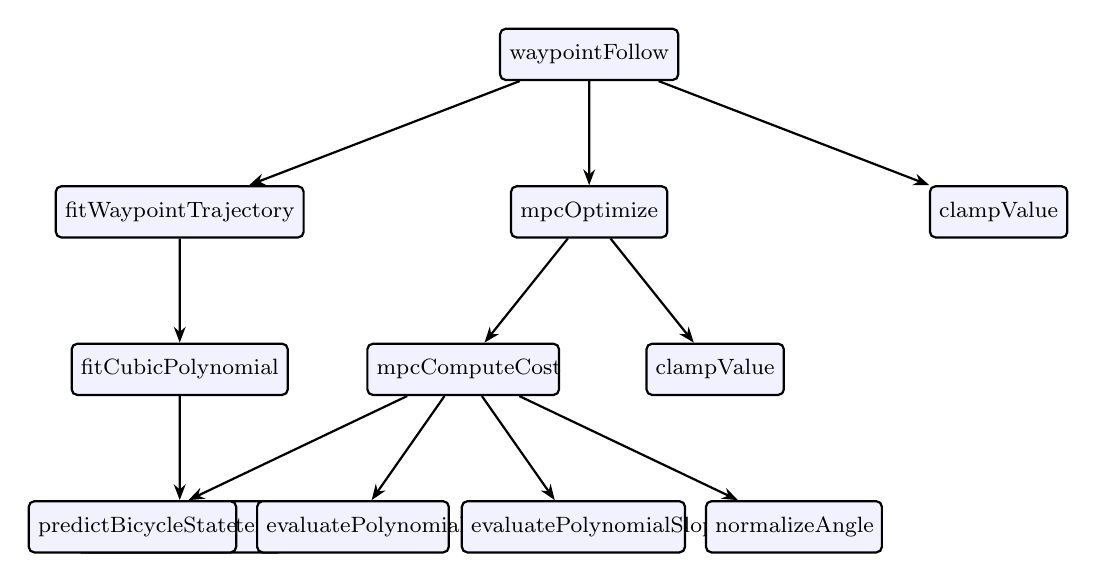
\begin{tikzpicture}[
  level 1/.style={sibling distance=5.2cm, level distance=2.0cm},
  level 2/.style={sibling distance=3.2cm, level distance=2.0cm},
  level 3/.style={sibling distance=2.8cm, level distance=2.0cm},
  every node/.style={rectangle, draw, rounded corners=2pt, thick,
    minimum height=0.65cm, text centered, font=\footnotesize,
    fill=blue!5},
  edge from parent/.style={draw, -{Stealth[length=2mm]}, thick}
]

\node {waypointFollow}
  child { node {fitWaypointTrajectory}
    child { node {fitCubicPolynomial}
      child { node {solveLinearSystem} }
    }
  }
  child { node {mpcOptimize}
    child { node[text width=2.2cm] {mpcComputeCost}
      child { node[text width=2.4cm] {predictBicycleState} }
      child { node[text width=2.2cm] {evaluatePolynomial} }
      child { node[text width=2.6cm] {evaluatePolynomialSlope} }
      child { node[text width=2.0cm] {normalizeAngle} }
    }
    child { node {clampValue} }
  }
  child { node {clampValue} };

\end{tikzpicture}
\end{center}

% ============================================================
%  7. 下级函数需求
% ============================================================
\section{下级函数需求}

\subsection{fitWaypointTrajectory~---~路点轨迹拟合}

\begin{itemize}
  \item \textbf{功能}：将原点与 6 个路点共 7 个数据点进行 X 归一化后三次多项式拟合，并估算参考车速。
  \item \textbf{输入}：\texttt{waypoints[6]}（Waypoint 数组）、\texttt{numWaypoints}（整数）、\texttt{egoSpeed}（double）。
  \item \textbf{输出}：\texttt{FittedTrajectory}（含多项式系数、归一化参数、参考车速、有效标志）。
  \item \textbf{算法}：X 坐标范围归一化 $\to$ Vandermonde 法方程 $\to$ 高斯消元求解系数。
  \item \textbf{异常处理}：X 方向跨度 $< 0.5$\,m 时标记为无效。
\end{itemize}

\subsection{mpcOptimize~---~MPC梯度下降优化器}

\begin{itemize}
  \item \textbf{功能}：采用中心差分数值梯度 + 自适应步长梯度下降优化 MPC 控制序列。
  \item \textbf{输入}：初始状态、参考轨迹、暖启动序列、上周期控制量、MPC 参数。
  \item \textbf{输出}：\texttt{MpcOptimizeOutput}（最优控制序列 + 最终代价值）。
  \item \textbf{算法}：计算所有分量梯度 $\to$ 归一化缩放 $\to$ 候选更新 $\to$ 约束投影 $\to$ 接受/衰减。
  \item \textbf{收敛}：最大迭代 30 次；学习率衰减因子 0.5。
\end{itemize}

\subsection{mpcComputeCost~---~MPC代价函数}

\begin{itemize}
  \item \textbf{功能}：计算给定控制序列下多步预测的 MPC 总代价。
  \item \textbf{输入}：控制序列、初始状态、参考轨迹、上周期控制量、MPC 参数。
  \item \textbf{输出}：double（总代价值）。
  \item \textbf{算法}：逐步预测 $\to$ 计算横向/航向/速度偏差 $\to$ 加权求和（含控制幅值与变化率代价）。
\end{itemize}

\subsection{clampValue~---~数值限幅截断}

\begin{itemize}
  \item \textbf{功能}：将数值截断到闭区间 $[\text{minVal}, \text{maxVal}]$。
  \item \textbf{输入}：\texttt{value}, \texttt{minVal}, \texttt{maxVal}（double）。
  \item \textbf{输出}：double（截断后的值）。
\end{itemize}

\subsection{fitCubicPolynomial~---~三次多项式拟合}

\begin{itemize}
  \item \textbf{功能}：对数据点进行三次多项式最小二乘拟合。
  \item \textbf{输入}：\texttt{xData[]}, \texttt{yData[]}（double 数组）、\texttt{numPoints}（整数）。
  \item \textbf{输出}：\texttt{PolynomialCoeffs}（4 个系数）。
  \item \textbf{算法}：构造 Vandermonde 矩阵的法方程 $(\mathbf{A}^{\!\top}\!\mathbf{A})\mathbf{c} = \mathbf{A}^{\!\top}\!\mathbf{y}$，调用高斯消元求解。
\end{itemize}

\subsection{evaluatePolynomial~---~多项式求值}

\begin{itemize}
  \item \textbf{功能}：使用 Horner 法计算 $y = c_0 + c_1 x + c_2 x^2 + c_3 x^3$。
  \item \textbf{输入}：\texttt{PolynomialCoeffs}、\texttt{x}（double）。
  \item \textbf{输出}：double（多项式值）。
\end{itemize}

\subsection{evaluatePolynomialSlope~---~多项式斜率求值}

\begin{itemize}
  \item \textbf{功能}：计算三次多项式一阶导数 $dy/dx = c_1 + 2c_2 x + 3c_3 x^2$。
  \item \textbf{输入}：\texttt{PolynomialCoeffs}、\texttt{x}（double）。
  \item \textbf{输出}：double（斜率值）。
\end{itemize}

\subsection{predictBicycleState~---~自行车模型状态预测}

\begin{itemize}
  \item \textbf{功能}：基于运动学自行车模型，使用欧拉前向离散预测下一时刻车辆状态。
  \item \textbf{输入}：\texttt{VehicleState}、\texttt{ControlInput}、\texttt{dt}、\texttt{wheelbase}（double）。
  \item \textbf{输出}：\texttt{VehicleState}（下一时刻状态）。
\end{itemize}

\subsection{normalizeAngle~---~角度归一化}

\begin{itemize}
  \item \textbf{功能}：将角度归一化到 $[-\pi, \pi]$ 区间，使用 $\text{atan2}(\sin\theta, \cos\theta)$。
  \item \textbf{输入}：\texttt{angle}（double）。
  \item \textbf{输出}：double（归一化后的角度）。
\end{itemize}

\subsection{solveLinearSystem~---~线性方程组求解}

\begin{itemize}
  \item \textbf{功能}：使用高斯消元法（部分主元选取）求解 $n \times n$ 线性方程组。
  \item \textbf{输入}：\texttt{matrix[]}（行主序矩阵，原位修改）、\texttt{rhs[]}（右端向量，原位存储解）、\texttt{n}、\texttt{maxDim}。
  \item \textbf{输出}：bool（是否求解成功）。
  \item \textbf{异常处理}：主元绝对值 $< 10^{-12}$ 时判定为奇异矩阵，返回 false。
\end{itemize}

% ============================================================
%  8. 数据结构定义
% ============================================================
\section{数据结构定义}

以下数据结构定义于 \texttt{waypointFollowTypes.hpp}，命名空间 \texttt{waypoint\_follow}。

\subsection{常量定义}

\begin{longtable}{|L{4.5cm}|C{1.5cm}|L{9cm}|}
\hline
\textbf{常量名} & \textbf{值} & \textbf{说明} \\
\hline
\endfirsthead
\hline
\textbf{常量名} & \textbf{值} & \textbf{说明} \\
\hline
\endhead
\texttt{NUM\_WAYPOINTS} & 6 & 参考路点数量 \\
\hline
\texttt{POLY\_COEFFS\_NUM} & 4 & 三次多项式系数数量 \\
\hline
\texttt{MAX\_PREDICTION\_HORIZON} & 30 & MPC最大预测步数 \\
\hline
\texttt{MAX\_CONTROL\_HORIZON} & 15 & MPC最大控制步数 \\
\hline
\texttt{MAX\_LINEAR\_SYSTEM\_DIM} & 8 & 线性方程组求解器最大维数 \\
\hline
\texttt{MIN\_SPEED\_THRESHOLD} & 0.5 & 控制器生效最低车速 (m/s) \\
\hline
\end{longtable}

\subsection{结构体定义}

\subsubsection{Waypoint~---~二维路点坐标}
\begin{longtable}{|L{3.5cm}|C{2cm}|L{9.5cm}|}
\hline
\textbf{成员} & \textbf{类型} & \textbf{说明} \\
\hline
\texttt{x} & double & 纵向坐标 (m)，自车坐标系前方为正 \\
\hline
\texttt{y} & double & 横向坐标 (m)，自车坐标系左方为正 \\
\hline
\end{longtable}

\subsubsection{PolynomialCoeffs~---~三次多项式系数}
\begin{longtable}{|L{3.5cm}|C{2cm}|L{9.5cm}|}
\hline
\textbf{成员} & \textbf{类型} & \textbf{说明} \\
\hline
\texttt{c[4]} & double[4] & $y = c_0 + c_1 x + c_2 x^2 + c_3 x^3$ \\
\hline
\end{longtable}

\subsubsection{FittedTrajectory~---~拟合参考轨迹}
\begin{longtable}{|L{3.5cm}|C{2cm}|L{9.5cm}|}
\hline
\textbf{成员} & \textbf{类型} & \textbf{说明} \\
\hline
\texttt{poly} & PolynomialCoeffs & 归一化坐标系下的多项式系数 \\
\hline
\texttt{xOffset} & double & X坐标归一化偏移量 (m) \\
\hline
\texttt{xScale} & double & X坐标归一化缩放因子 (m) \\
\hline
\texttt{refSpeed} & double & 路点推算的参考车速 (m/s) \\
\hline
\texttt{valid} & bool & 轨迹拟合是否有效 \\
\hline
\end{longtable}

\subsubsection{VehicleState~---~车辆运动状态}
\begin{longtable}{|L{3.5cm}|C{2cm}|L{9.5cm}|}
\hline
\textbf{成员} & \textbf{类型} & \textbf{说明} \\
\hline
\texttt{x} & double & 纵向位置 (m) \\
\hline
\texttt{y} & double & 横向位置 (m) \\
\hline
\texttt{yaw} & double & 航向角 (rad)，逆时针为正 \\
\hline
\texttt{v} & double & 纵向速度 (m/s) \\
\hline
\end{longtable}

\subsubsection{ControlInput~---~车辆控制输入量}
\begin{longtable}{|L{3.5cm}|C{2cm}|L{9.5cm}|}
\hline
\textbf{成员} & \textbf{类型} & \textbf{说明} \\
\hline
\texttt{steeringAngle} & double & 前轮转向角 (rad)，左转为正 \\
\hline
\texttt{acceleration} & double & 纵向加速度 (m/s\textsuperscript{2})，加速为正 \\
\hline
\end{longtable}

\subsubsection{MpcParam~---~MPC控制参数集}
\begin{longtable}{|L{4cm}|C{1.5cm}|C{1.5cm}|L{8cm}|}
\hline
\textbf{成员} & \textbf{类型} & \textbf{默认值} & \textbf{说明} \\
\hline
\endfirsthead
\hline
\textbf{成员} & \textbf{类型} & \textbf{默认值} & \textbf{说明} \\
\hline
\endhead
\texttt{predictionHorizon} & int & 15 & 预测步数 \\
\hline
\texttt{controlHorizon} & int & 5 & 控制步数 \\
\hline
\texttt{dt} & double & 0.1 & 预测时间步长 (s) \\
\hline
\texttt{wheelbase} & double & 2.85 & 前后轴距 (m) \\
\hline
\texttt{maxSteeringAngle} & double & 0.5236 & 前轮最大转向角 (rad) \\
\hline
\texttt{maxAcceleration} & double & 3.0 & 最大纵向加速度 (m/s\textsuperscript{2}) \\
\hline
\texttt{minAcceleration} & double & --5.0 & 最大纵向减速度 (m/s\textsuperscript{2}) \\
\hline
\texttt{maxSteeringRate} & double & 0.05 & 每步最大转向角变化量 (rad/step) \\
\hline
\texttt{wLateral} & double & 50.0 & 横向偏差代价权重 \\
\hline
\texttt{wHeading} & double & 30.0 & 航向偏差代价权重 \\
\hline
\texttt{wVelocity} & double & 5.0 & 速度偏差代价权重 \\
\hline
\texttt{wSteering} & double & 1.0 & 转向角控制量代价权重 \\
\hline
\texttt{wAccel} & double & 0.5 & 加速度控制量代价权重 \\
\hline
\texttt{wSteeringRate} & double & 100.0 & 转向角变化率代价权重 \\
\hline
\texttt{wAccelRate} & double & 10.0 & 加速度变化率代价权重 \\
\hline
\texttt{maxOptIterations} & int & 30 & 梯度下降最大迭代次数 \\
\hline
\texttt{learningRate} & double & 0.5 & 梯度下降初始学习率 \\
\hline
\texttt{finiteDiffEps} & double & $10^{-3}$ & 中心差分步长 \\
\hline
\end{longtable}

\subsubsection{WaypointFollowInput~---~控制器输入}
\begin{longtable}{|L{4.5cm}|C{2.5cm}|L{8cm}|}
\hline
\textbf{成员} & \textbf{类型} & \textbf{说明} \\
\hline
\texttt{egoSpeed} & double & 自车车速 (m/s) \\
\hline
\texttt{currentSteeringWheelAngle} & double & 当前方向盘转角 (rad) \\
\hline
\texttt{waypoints[6]} & Waypoint[6] & 参考路点，对应未来 0.5/1.0/.../3.0\,s \\
\hline
\end{longtable}

\subsubsection{WaypointFollowOutput~---~控制器输出}
\begin{longtable}{|L{4.5cm}|C{2.5cm}|L{8cm}|}
\hline
\textbf{成员} & \textbf{类型} & \textbf{说明} \\
\hline
\texttt{steeringWheelAngle} & double & 目标方向盘转角 (rad) \\
\hline
\texttt{acceleration} & double & 目标纵向加速度 (m/s\textsuperscript{2}) \\
\hline
\end{longtable}

\subsubsection{WaypointFollowParam~---~控制器参数}
\begin{longtable}{|L{4.5cm}|C{2.5cm}|L{8cm}|}
\hline
\textbf{成员} & \textbf{类型} & \textbf{说明} \\
\hline
\texttt{mpcParam} & MpcParam & MPC控制参数集 \\
\hline
\texttt{steeringRatio} & double & 方向盘到前轮转角传动比（默认 15.0） \\
\hline
\end{longtable}

\subsubsection{WaypointFollowState~---~控制器状态}
\begin{longtable}{|L{4.5cm}|C{2.8cm}|L{7.7cm}|}
\hline
\textbf{成员} & \textbf{类型} & \textbf{说明} \\
\hline
\texttt{prevControlSequence[15]} & ControlInput[15] & 上一周期MPC控制序列（暖启动） \\
\hline
\texttt{lastAppliedControl} & ControlInput & 上一周期实际施加的控制量 \\
\hline
\texttt{initialized} & bool & 暖启动状态是否已初始化 \\
\hline
\end{longtable}

\subsubsection{MpcOptimizeOutput~---~优化器输出}
\begin{longtable}{|L{4.5cm}|C{2.8cm}|L{7.7cm}|}
\hline
\textbf{成员} & \textbf{类型} & \textbf{说明} \\
\hline
\texttt{optimalSequence[15]} & ControlInput[15] & 优化后的控制序列 \\
\hline
\texttt{finalCost} & double & 优化后的代价值 \\
\hline
\end{longtable}

% ============================================================
%  9. 测试用例
% ============================================================
\section{测试用例}

\subsection{正常测试用例}

{\small
\begin{longtable}{|C{0.6cm}|L{2.2cm}|L{4.8cm}|L{4.0cm}|L{3.5cm}|}
\hline
\textbf{编号} & \textbf{场景} & \textbf{输入} & \textbf{预期输出} & \textbf{验证准则} \\
\hline
\endfirsthead
\hline
\textbf{编号} & \textbf{场景} & \textbf{输入} & \textbf{预期输出} & \textbf{验证准则} \\
\hline
\endhead
N-1 &
直线行驶 &
$v{=}20$, $\theta_{\text{sw}}{=}0$, 路点沿 $y{=}0$ 直线均匀分布 &
$\theta_{\text{sw}}^* \approx 0$, $a^* \approx 0$ &
$|\theta_{\text{sw}}^*| < 0.01$\,rad, $|a^*| < 0.5$ \\
\hline
N-2 &
恒定左转弯 &
$v{=}15$, $\theta_{\text{sw}}{=}0$, 路点沿圆弧（$R{=}100$\,m）分布 &
$\theta_{\text{sw}}^* > 0$（左转） &
$\theta_{\text{sw}}^*$ 方向正确且幅值合理 \\
\hline
N-3 &
S形变道 &
$v{=}18$, $\theta_{\text{sw}}{=}0$, 路点构成 S 形轨迹 &
$\theta_{\text{sw}}^*$ 先左后右, $a^*$ 合理 &
输出在物理约束范围内 \\
\hline
N-4 &
巡航加速 &
$v{=}10$, 路点按 $v_{\text{ref}}{=}15$ 间距分布 &
$a^* > 0$（加速） &
$a^* > 0$ 且 $\leq a_{\max}$ \\
\hline
N-5 &
暖启动连续调用 &
连续两次调用, 第一次初始化, 第二次利用暖启动 &
第二次输出平滑, 代价值不高于冷启动 &
两次输出转向角变化 $< \Delta\delta_{\max} \cdot r_{\text{steer}}$ \\
\hline
\end{longtable}
}

\vspace{6pt}
{\small
\begin{longtable}{|L{2.5cm}|L{13cm}|}
\hline
\multicolumn{2}{|c|}{\textbf{正常测试用例符号说明}} \\
\hline
\textbf{符号} & \textbf{含义} \\
\hline
$v$ & 自车车速 egoSpeed (m/s) \\
\hline
$\theta_{\text{sw}}$ & 当前方向盘转角 currentSteeringWheelAngle (rad) \\
\hline
$\theta_{\text{sw}}^*$ & 输出目标方向盘转角 steeringWheelAngle (rad) \\
\hline
$a^*$ & 输出目标加速度 acceleration (m/s\textsuperscript{2}) \\
\hline
$R$ & 圆弧半径 (m) \\
\hline
$v_{\text{ref}}$ & 参考车速 (m/s) \\
\hline
$a_{\max}$ & 最大纵向加速度 maxAcceleration (m/s\textsuperscript{2}) \\
\hline
$\Delta\delta_{\max}$ & 每步最大转向角变化量 maxSteeringRate (rad/step) \\
\hline
$r_{\text{steer}}$ & 方向盘到前轮传动比 steeringRatio \\
\hline
\end{longtable}
}

\subsection{异常测试用例}

{\small
\begin{longtable}{|C{0.6cm}|L{2.0cm}|L{4.5cm}|L{4.2cm}|L{3.8cm}|}
\hline
\textbf{编号} & \textbf{场景} & \textbf{输入} & \textbf{预期输出/行为} & \textbf{验证准则} \\
\hline
\endfirsthead
\hline
\textbf{编号} & \textbf{场景} & \textbf{输入} & \textbf{预期输出/行为} & \textbf{验证准则} \\
\hline
\endhead
A-1 &
零速保护 &
$v{=}0$, 路点正常 &
$\theta_{\text{sw}}^* = \theta_{\text{sw}}$, $a^*{=}0$ &
低速保护分支激活 \\
\hline
A-2 &
极低速 &
$v{=}0.49$\,m/s（阈值下沿） &
$\theta_{\text{sw}}^* = \theta_{\text{sw}}$, $a^*{=}0$ &
$v < 0.5$ 时不进入优化 \\
\hline
A-3 &
NaN 车速 &
$v{=}\text{NaN}$, 路点正常 &
不崩溃; 输出有限值或安全保护值 &
函数返回, 无浮点异常 \\
\hline
A-4 &
Infinity 车速 &
$v{=}+\infty$, 路点正常 &
不崩溃; 输出限幅范围内 &
$|\theta_{\text{sw}}^*| \leq \delta_{\max} r_s$, $a_{\min} \leq a^* \leq a_{\max}$ \\
\hline
A-5 &
路点全重合 &
6 个路点坐标全为 $(0,0)$ &
拟合无效, 输出零控制 &
\texttt{valid == false}, 零控制输出 \\
\hline
A-6 &
路点 X 跨度过小 &
所有路点 $x \in [0, 0.3]$（$< 0.5$\,m） &
拟合无效, 输出保持当前状态 &
\texttt{valid == false} \\
\hline
A-7 &
极限曲率路点 &
路点构成极小半径（$R{=}2$\,m）急弯 &
输出被限幅到 $\pm\delta_{\max} \cdot r_s$ &
转向角不超过物理极限 \\
\hline
A-8 &
NaN 路点坐标 &
\texttt{waypoints[2].y = NaN}, 其余正常 &
不崩溃; 拟合可能失败 &
函数正常返回 \\
\hline
A-9 &
负速度输入 &
$v{=}{-}5$\,m/s &
低速保护激活（$v < 0.5$） &
$\theta_{\text{sw}}^* = \theta_{\text{sw}}$, $a^*{=}0$ \\
\hline
A-10 &
方向盘转角饱和 &
$\theta_{\text{sw}}{=}10$\,rad, $v{=}15$, 路点正常 &
输出 $\theta_{\text{sw}}^*$ 被限幅 &
$|\theta_{\text{sw}}^*| \leq \delta_{\max} \cdot r_s$ \\
\hline
\end{longtable}
}

\vspace{6pt}
{\small
\begin{longtable}{|L{2.5cm}|L{13cm}|}
\hline
\multicolumn{2}{|c|}{\textbf{异常测试用例符号说明}} \\
\hline
\textbf{符号} & \textbf{含义} \\
\hline
$v$ & 自车车速 egoSpeed (m/s) \\
\hline
$\theta_{\text{sw}}$ & 当前方向盘转角 currentSteeringWheelAngle (rad) \\
\hline
$\theta_{\text{sw}}^*$ & 输出目标方向盘转角 steeringWheelAngle (rad) \\
\hline
$a^*$ & 输出目标加速度 acceleration (m/s\textsuperscript{2}) \\
\hline
$\delta_{\max}$ & 前轮最大转向角 maxSteeringAngle (rad) \\
\hline
$r_s$ & 方向盘到前轮传动比 steeringRatio \\
\hline
$a_{\min}$, $a_{\max}$ & 最小/最大纵向加速度 (m/s\textsuperscript{2}) \\
\hline
$R$ & 路点构成的等效转弯半径 (m) \\
\hline
NaN & IEEE 754 非数值 (Not a Number) \\
\hline
$+\infty$ & IEEE 754 正无穷大 \\
\hline
\end{longtable}
}

\end{document}
